\documentclass[10pt,a4paper]{beamer}
\usepackage[utf8]{inputenc}
\usepackage[frenchb]{babel}
\usepackage[T1]{fontenc}
\usetheme{Madrid}
\usepackage{amsmath}
\usepackage{courier}
\usepackage{times}
\usepackage{amsfonts}
\usepackage{amssymb}
\usepackage{makeidx}
\usepackage{graphicx}
\usepackage{lmodern}
\usepackage{kpfonts}
\usepackage[osf]{garamondx}
\usefonttheme{serif}
\usepackage{listings}
\usepackage{tikz}
\usepackage{atbegshi}
\usepackage{eso-pic}
\usepackage{caption}
\usepackage{verbatim}
\usepackage{hyperref}
\definecolor{blueclair}{rgb}{0.9, 0.992, 252}
\definecolor{bluefonce}{rgb}{0, 0.2, 0.4}

\definecolor{colKeys}{rgb}{0, 0, 1}
\definecolor{colIdentifier}{rgb}{0, 0, 0}
\definecolor{colString}{rgb}{0.6, 0.1, 0.1}
%Permet d'utiliser les code dans les diapositives : Ne peinez pas à demander google.
\lstnewenvironment{sql}
	{%\inputencoding{}
	\lstset{		
		language=SQL,
		basicstyle=\footnotesize\ttfamily,
		numbers=left,
		keywordstyle=\color{colKeys},
		commentstyle=\color{gray}\it ,
		identifierstyle=\color{bluefonce},
		stringstyle=\color{colString},
		numberstyle=\scriptsize,
		stepnumber=1,
		numbersep=5pt,
		showstringspaces=false,
		xrightmargin=1cm,
		frameround=tttt,
		extendedchars=true,%accents dans le code
		backgroundcolor=\color{yellow!20},
		breaklines=true,
		frame=l
	}
}{}

\makeatletter
	\lst@AddToHook{TextStyle}{\let\lst@basicstyle\ttfamily\normalsize\fontfamily{cmss}\selectfont}
\makeatother


\setbeamertemplate{footline}
{
  \leavevmode%
  \hbox{%
  \begin{beamercolorbox}[wd=.333333\paperwidth, ht=2.25ex,dp=1ex,center]{author in head/foot}%
    \usebeamerfont{author in head/foot}\insertshortauthor%~~\beamer@ifempty{\insertshortinstitute}{}{(\insertshortinstitute)}
  \end{beamercolorbox}%
  \begin{beamercolorbox}[wd=.333333\paperwidth, ht=2.25ex,dp=1ex,center]{title in head/foot}%
    \usebeamerfont{title in head/foot}{\bf Titre en pied de page }
  \end{beamercolorbox}%
  \begin{beamercolorbox}[wd=.333333\paperwidth, ht=2.25ex,dp=1ex,right]{date in head/foot}%
    \usebeamerfont{date in head/foot}\insertshortdate{\today}\hspace*{2em}
    \insertframenumber{} / \inserttotalframenumber\hspace*{2ex} 
  \end{beamercolorbox}}%
  \vskip0pt%  
}
\makeatother

%Profondeur de la table des matières (sommaire de la présentation)
\setcounter{tocdepth}{2}

\defbeamertemplate*{headline}{myHeadline}
{%
  \begin{beamercolorbox}[ht=2.5ex,dp=2ex]{section in head/foot}%
    \insertsectionnavigationhorizontal{\paperwidth}{}{}%
  \end{beamercolorbox}%
  \begin{beamercolorbox}[ht=2.875ex,dp=0.75ex]{subsection in head/foot}
    \usebeamerfont{subsection in head/foot}
    \insertsubsectionnavigationhorizontal{\paperwidth}{}{\hskip0pt plus1filll%
    \hskip2ex}%
  \end{beamercolorbox}%
}

\setbeamertemplate{note page}[plain]

%\date{25 Mars 2013}
\newcommand{\filigrane}{
\begin{tikzpicture}[remember picture, overlay]
	\node[text opacity=0.8]
	at (current page.center){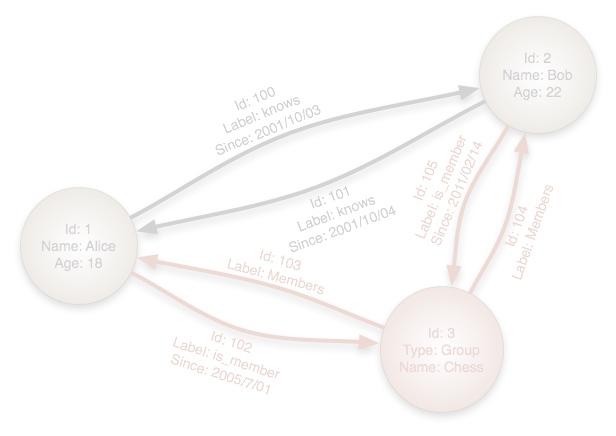
\includegraphics[scale=0.6]{images/graph_rapport}};
\end{tikzpicture}
%}
}
\setbeamertemplate{background}[grid][step=0.5cm]

\def\colorize<#1>{%
\temporal<#1>{\color{red!50}\small}{\color{black}\Large}{\color{black!50}}}

\title{\bf\scshape {\Huge GRAND TITRE } : PLUS D'EXPLICATIONS }
\subtitle{\it Sous titre }
\author[\bf Koffi Sani]{{\bf \LARGE Koffi Sani} \\ {\it  Ingénieur Concepteur en Informatique}}
%\institute{2$^{\grave{e}me}$ Année Ingénieur\\ Année académique 2012-2013}
\date{}
\setbeamercovered{transparent}	

\def\colorize<#1>{%
\temporal<#1>{\color{red!50}\small}{\color{black}\Large}{\color{black!50}}}
%\rightlogo[0.9]{../mon_memoire/images/logo_iai.jpg}

\begin{document}
\setbeamertemplate{background canvas}{\filigrane}
\shorthandoff{!}
% désactiver le « ! » (babel/frenchb)
\newcount\opaqueness % pour variation de la couleur
\newcount\offset
% pour le déplacement latéral
\transduration{1}
\frame
{

\center
	\begin{minipage}{70mm}
		
		%\begin{exampleblock}{}
			\center{
\includegraphics[scale=0.04]{images/logo_iai.jpg}}
			\begin{center}
			{\bf \footnotesize Institut Africain d'Informatique}\\
			\scriptsize{ \it Etablissement Inter-Etats d'Enseignement Supérieur }\\
			B.P. 2263 Libreville, GABON\\
			Tél. : (+241) 07 70 55 00 / 07 70 56 00 \\
			Site web : www.iaisiege.com \quad E-mail : contact@iaisiege.com
			\end{center}
		%\end{exampleblock}
	\end{minipage}\transdissolve
	\maketitle \vspace{-1.5cm}
	%\begin{center}
	
	%Sous la supervision de 
	%\bf Dr Ange NAMBILA
	%\end{center}
	
}
\logo{
	
\includegraphics[height=0.7cm]{images/logo_iai.jpg}
	\hspace{\dimexpr\paperwidth-2cm-5pt}
	
\includegraphics[height=0.7cm]{images/logo_iai.jpg}
	}

\frame{\frametitle{Sommaire}
\tableofcontents\transdissolve
}
\AtBeginSection[currentsection, currentsubsection, hideothersubsection, sectionstyle=show/hide, subsectionstyle=show/shade] % Do nothing for \section*
{\transblindshorizontal
	\begin{frame}<beamer>
		\transdissolve
		\frametitle{Plan de l'exposé}
		\tableofcontents[currentsection, hideothersubsections]%, pausesubsections]
	\end{frame}
}

\section{Première section}
\subsection{Première sous-section}
\frame{

}
\subsection{Deuxième sous-section}
\frame{

}

\section{Deuxième section}
\frame{
}
\end{document}